\documentclass{article}

\usepackage{authblk}
\usepackage{multirow}

\usepackage{graphicx}
\usepackage{subcaption}

%\usepackage{amsmath}


\usepackage{geometry}
 \geometry{
		a4paper,
		left=22mm,
		right=22mm,
		top=20mm,
		bottom=20mm
	}

\title{Analyzing Performance of \\Matrix Multiplication Algorithms in OpenMP}
\author{R Mukesh (CED15I002)}
\affil{IIITDM Kancheepuram}
\date{August 26, 2018}

\begin{document}
\maketitle

\begin{abstract}
	Parallelism is the key to improving performance of algorithms. This experiment aims to analyze the performance of parallelized matrix multiplication algorithms in OpenMP, for various matrix storage schemes (row-major, column-major and block matrix storage order).
\end{abstract}

\section{Results \protect\footnote{The experiments were conducted on a computer with 6\textsuperscript{th} Generation Intel(R) Core(TM) i7-6500U Processor (4M Cache, upto 3.10 GHz) and 4GB Single Channel DDR3L 1600M Hz (4GBx1) RAM.}}

The experiments were performed on double datatype matrices with a dimension of 2048 x 2048 elements. The block size of the block-order matrices was taken as 4 x 4 elements.

\begin{table}[!htbp]
\begin{tabular}{|c|c|c|c|l}
\cline{1-4}
\multirow{2}{*}{\textbf{Number of Threads}} & \multicolumn{3}{c|}{\textbf{Execution Time (in seconds)}} &  \\ \cline{2-4}
 & \textbf{Row-Major Matrix} & \textbf{Column-Major Matrix} & \textbf{Block-Order Matrix} &  \\ \cline{1-4}
Without OpenMP & 39.623860 & 39.434041 & 49.235846 &  \\ \cline{1-4}
1 & 49.994157 & 50.452567 & 49.811989 &  \\ \cline{1-4}
2 & 26.935359 & 27.512718 & 25.561742 &  \\ \cline{1-4}
4 & 24.656942 & 24.657366 & 24.169181 &  \\ \cline{1-4}
6 & 24.793141 & 24.703847 & 24.635781 &  \\ \cline{1-4}
8 & 24.742557 & 24.767288 & 24.672302 &  \\ \cline{1-4}
10 & 24.682174 & 24.731551 & 24.779522 &  \\ \cline{1-4}
12 & 24.662531 & 24.803336 & 24.766994 &  \\ \cline{1-4}
16 & 24.713110 & 24.986742 & 24.749395 &  \\ \cline{1-4}
20 & 24.701823 & 24.862698 & 25.155818 &  \\ \cline{1-4}
24 & 24.748892 & 24.868193 & 25.022288 &  \\ \cline{1-4}
28 & 24.765814 & 24.891739 & 24.972449 &  \\ \cline{1-4}
32 & 24.770109 & 24.860866 & 24.869343 &  \\ \cline{1-4}
\end{tabular}
\end{table}

\begin{figure}[!htbp]

	\centering
	\begin{subfigure}[!htbp]{\textwidth}
		\centering
		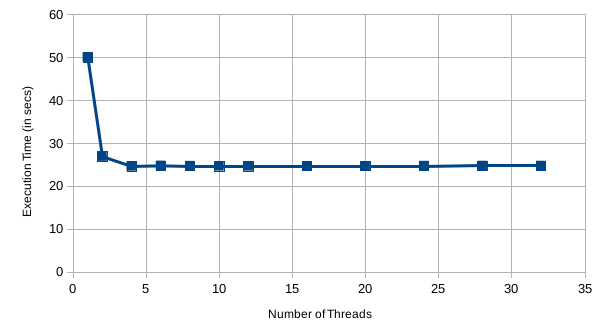
\includegraphics[scale=0.8]{rowmajorperformance}
		\subcaption{Performance of Row-Major Matrix Multiplication}
	\end{subfigure}
	
	\begin{subfigure}[!htbp]{\textwidth}
		\centering
		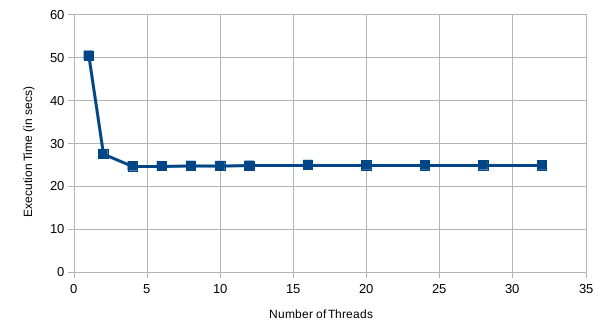
\includegraphics[scale=0.8]{columnmajorperformance}
		\subcaption{Performance of Column-Major Matrix Multiplication}
	\end{subfigure}
	
	\begin{subfigure}[!htbp]{\textwidth}
		\centering
		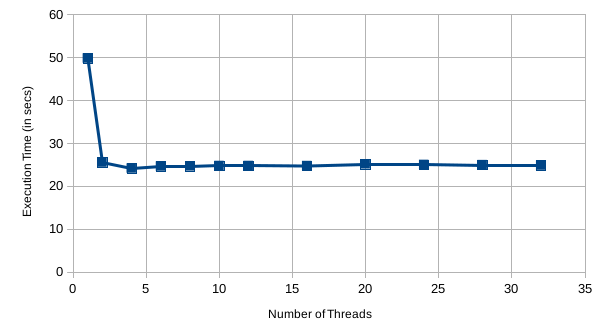
\includegraphics[scale=0.8]{blockorderperformance}
		\subcaption{Performance of Block Matrix Multiplication}
	\end{subfigure}
	
	\caption{Number of Threads vs Execution Time of Row-Major, Column-Major and Block Matrix Multiplication in OpenMP}
\end{figure}

\section{Calculation}

The parallel fraction of the algorithm can be computed using the following equation:

\begin{equation}
	f = \frac{(1-T_p/T_1)}{(1-1/p)}
\end{equation}

For Row-Major Matrix Multiplication Algorithm, 
\[f = \frac{(1-24.656942/49.994157)}{(1-1/4)} = \textbf{0.675738033 (67.57\%)}\]

For Column-Major Matrix Multiplication Algorithm, 
\[f = \frac{(1-24.657366/50.452567)}{(1-1/4)} = \textbf{0.681701713 (68.17\%)}\]

For Block Matrix Multiplication Algorithm, 
\[f = \frac{(1-24.169181/49.811989)}{(1-1/4)} = \textbf{0.686389188 (68.63\%)}\]

\section{Inferences}

\begin{enumerate}
	\item The matrix multiplication algorithms for the various matrix storage schemes (row-Major, column-Major and block-order) have same parallel fraction (f) of approximately 68\%.
	
	\item The execution time of matrix multiplication algorithms drops until the number of threads is 4 and then saturates as the computer hardware has only four cores and therefore supports only four simaltaneous threads.
	
	\item The slight increase in execution time for number of threads beyond four is attributed to the overheads associated with creation and switching of threads.
	
	\item The slightly improved performance of block matrix multiplication over row-major and column-major matrix multiplication is due the reduced number of cache misses that can be attributed to the memory access patterns of the algorithm.
	
\end{enumerate}

\end{document}